%!TEX root = ../main.tex

\chapter{\texorpdfstring{$\CP$}{CP} Violation}
\label{sec:cpviolation}

In this chapter the concept of \CP violation, its origin and manifestation in
the SM, as well as the possibilities to measure \CP violation, are described.
The formalism closely follows Refs.~\cite{Harrison:1998yr} and
\cite{Branco:1999fs}.

%!TEX root = ../main.tex

\section{The KM mechanism and the CKM matrix (4 pages)}
\label{sec:cpviolation:kmmechanism}

Quarks get their mass through coupling to the Higgs field with vacuum
expectation value $v$ and via Yukawa interaction between the left-handed and
the right-handed quark content. The Yukawa matrices $\matr{Y}_d$ and
$\matr{Y}_u$ for down-type and up-type quarks involved in the corresponding
Lagrangian
\begin{align}
	\mathcal{L}_{\textrm{Yukawa}} = - \frac{v}{\sqrt{2}} (\bar{d}_{\mathrm{L}} \matr{Y}_d d_{\mathrm{R}} + \bar{u}_{\mathrm{L}} \matr{Y}_u u_{\mathrm{R}}) + \text{h.c.}
\end{align}
are not necessarily diagonal. The mass eigenstates $q^{\prime}$ can be
obtained by a unitary transformation
\begin{align}
	q^{\prime}_{\mathrm{A}} = \matr{V}_{\mathrm{A,}q}q_{\mathrm{A}} \quad \text{for } q = u,d \text{ and } \mathrm{A} = \mathrm{L,R}
\end{align}
with $\matr{V}_{\mathrm{A,}q}\matr{V}^\dagger_{\mathrm{A,}q} = 1$. When
applying this transformation in the Lagrangian that describes the
charged-current interaction
\begin{align}
	\mathcal{L}_{\textrm{CC}} &= -\frac{g_2}{\sqrt{2}}(\bar{u}_{\mathrm{L}}\gamma^{\mu}W_{\mu}^+ d_{\mathrm{L}} + \bar{d}_{\mathrm{L}}\gamma^{\mu}W_{\mu}^-u_{\mathrm{L}})\\
	&= -\frac{g_2}{\sqrt{2}}(\bar{u}^\prime_{\mathrm{L}}\gamma^{\mu}W_{\mu}^+\matr{V}_{\mathrm{L,}u}\matr{V}^\dagger_{\mathrm{L,}d}d^\prime_{\mathrm{L}} + \bar{d}^\prime_{\mathrm{L}}\gamma^{\mu}W_{\mu}^-\matr{V}_{\mathrm{L,}d}\matr{V}^\dagger_{\mathrm{L,}u}u^\prime_{\mathrm{L}})
\end{align}
the Cabibbo-Kobayashi-Maskawa matrix $\matr{V}_{\text{CKM}} =
\matr{V}_{\mathrm{L,}u}\matr{V}^\dagger_{\mathrm{L,}d}$ enters. As the
Yukawa matrices are not diagonalised by the same unitary transformation, the
CKM matrix is not the unit matrix and thus allows for flavour changes in the
weak interaction. So, the CKM matrix can be understood as the connection
between the mass eigenstates and the eigenstates to the weak interaction
\begin{align}
\begin{pmatrix}
d^\prime \\ s^\prime \\ b^\prime
\end{pmatrix}
=
\begin{pmatrix}
\Vud & \Vus & \Vub \\
\Vcd & \Vcs & \Vcb \\
\Vtd & \Vts & \Vtb \\
\end{pmatrix}
\begin{pmatrix}
d	\\	s	\\	b
\end{pmatrix}
\end{align}
Being the product of two unitary matrices the CKM matrix itself is unitary as
well. In general, a complex $3\times3$ matrix has 18 free parameters. However,
the unitarity removes nine of the degrees of freedom. Another five phases can
be constrained by global rephasings between the six mass fields. So, four free
parameters remain, of which three are real-valued angles and one is a complex
phase. This single phase introduces \CP violation to the SM. Kobayashi and
Maskawa developed this concept, which explains the origin of \CP violation and
predicted the existence of the third quark generation~\cite{Kobayashi:1973fv}.
The corresponding parametrisation of the CKM matrix is
\begin{align}
\matr{V}_{\text{CKM}} =
\begin{pmatrix}
c_1 & -s_1c_3 & -s_1s_3 \\
s_1c_2 & c_1c_2c_3 - s_2s_3e^{i\delta} & c_1c_2s_3 + s_2c_3e^{i\delta} \\
s_1s_2 & c_1s_2c_3 + c_2s_3e^{i\delta} & c_1s_2s_3 - c_2c_3e^{i\delta}
\end{pmatrix}
\,,
\end{align}
with $c_i$ and $s_i$ being shorthand for the cosine respectively sine of the
three Euler angles, and $\delta$ is the irreducible phase. Tests of the SM
concerning \CP violation in the quark mixing sector are performed by examining
the unitarity conditions of the CKM matrix. Six of the 12 equations are
orthogonality relations, which can be interpreted as triangles in the complex
plane. The area of all triangles is the same and given by half of the Jarlskog
invariant
\begin{align}
	J_{\CP} = \pm\,\mathcal{I}m (V_{ik}^{}V_{jl}^{}V_{il}^{\ast}V_{jk}^{\ast}) \quad (i \neq j, l \neq k)\,,
\end{align}
which expresses the amount of \CP violation in the
SM~\cite{Jarlskog:1985ht,*Jarlskog:1985cw}. It is measured to be $J = (3.04
^{+0.21}_{-0.20}) \times\num{e-5}$~\cite{PDG2016}. However, the ratios of the
side lengths of the unitarity triangles are very different. In two of them all
sides are of comparable length, one of the conditions is given by
\begin{align}
	\Vud\Vubs + \Vcd\Vcbs + \Vtd\Vtbs = 0\,.
\end{align}
When depicting the triangle in the complex plane it is convenient to scale the
triangle by dividing all side lengths by $\Vcd\Vcbs$. Then, the base matches
the real axis with length one as can be seen in
\cref{fig:cpviolation:ckmtriangle}.
\begin{figure}[htb]
\centering
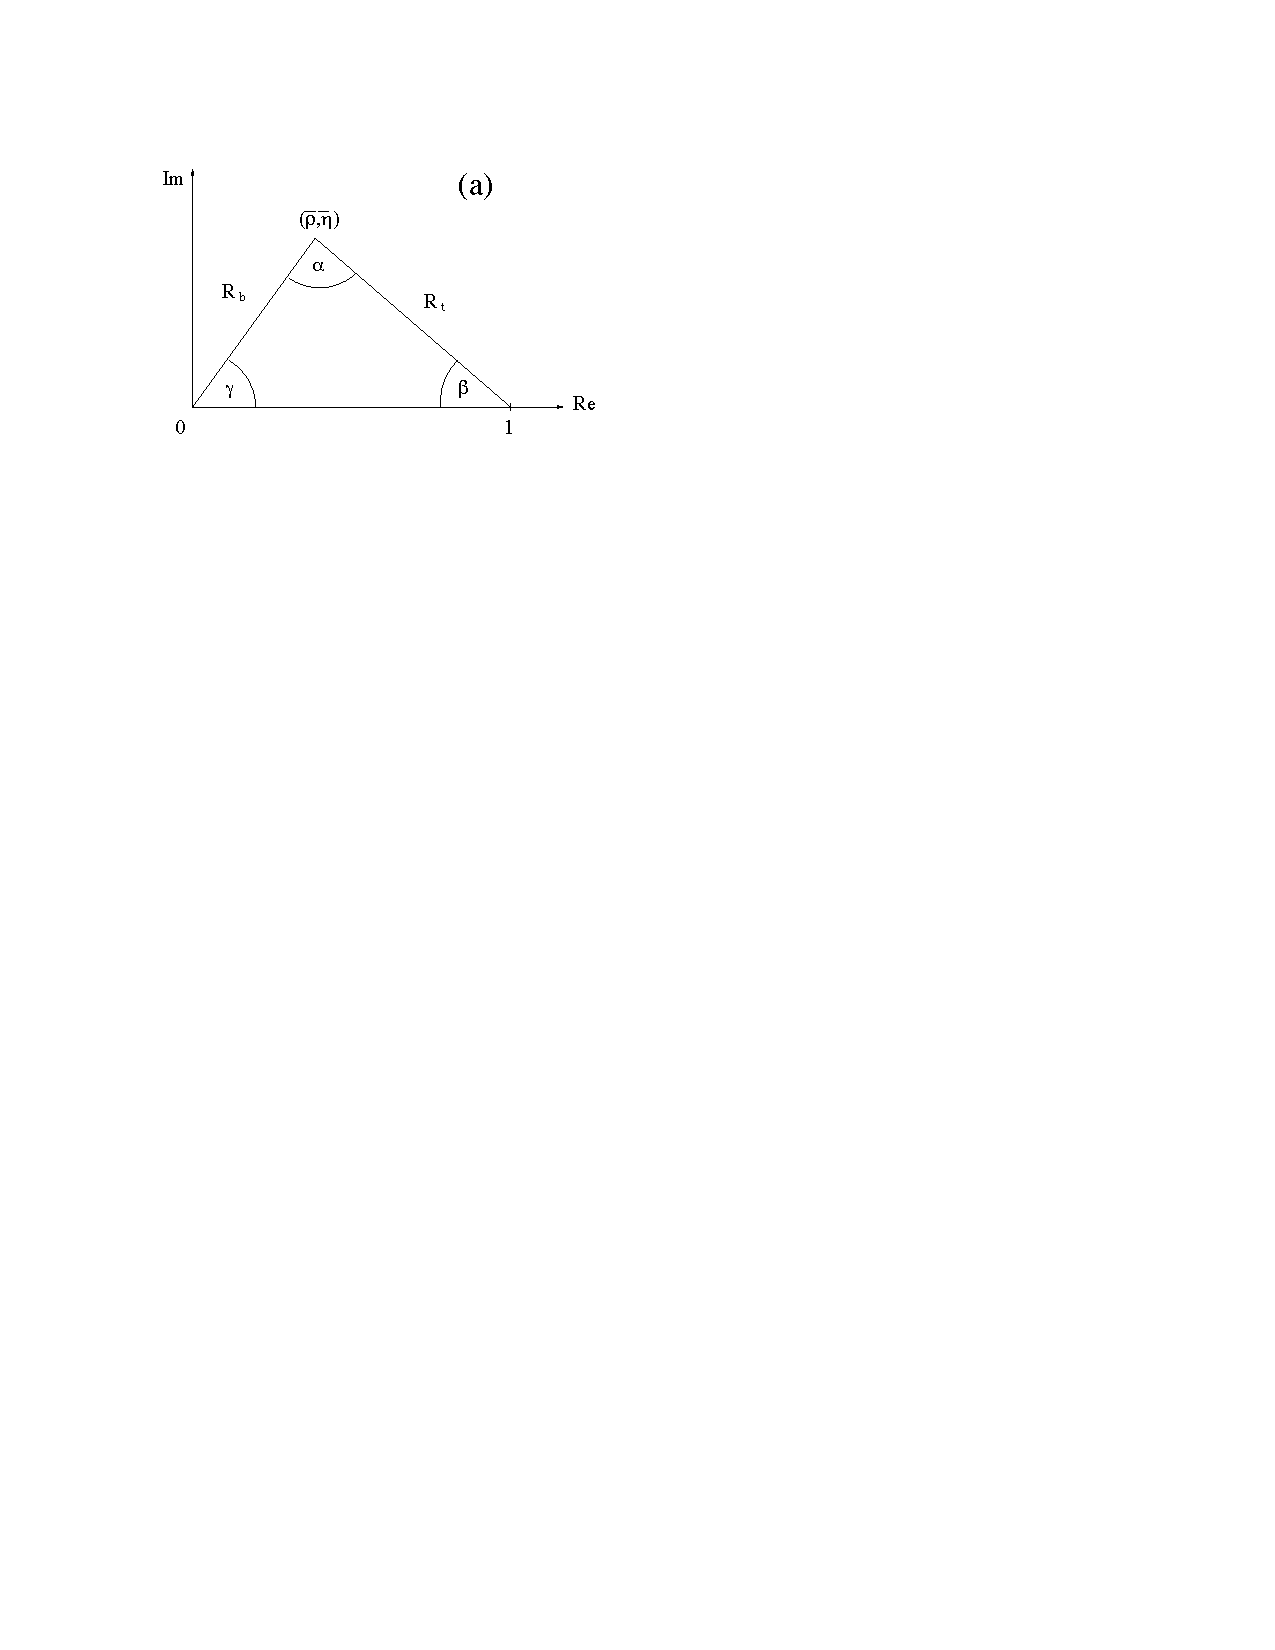
\includegraphics[width=0.5\textwidth]{03-CPViolation/figs/CKMtriangle_prelim.pdf}
\caption{Schematic representation of the CKM unitarity triangle.}
\label{fig:cpviolation:ckmtriangle}
\end{figure}
\todo{replace CKM triangle by self-made version}
Using the parametrisation of the CKM matrix by
Wolfenstein~\cite{Wolfenstein:1983yz}, which is an expansion in powers of
$\lambda \equiv |\Vus| = \num{0.2248\pm0.0006}$~\cite{PDG2016}
\begin{align}
\matr{V}_{\text{CKM}} =
\begin{pmatrix}
1 - \frac 12 \lambda^2 & \lambda & A\lambda^3(\rho - i\eta) \\
- \lambda & 1 - \frac 12 \lambda^2 & A\lambda^2 \\
A\lambda^3(1 - \rho - i\eta) & -A\lambda^2 & 1
\end{pmatrix}
+ \mathcal{O}(\lambda^4)
\end{align}
the other two sides are given by
\begin{align}
	R_b &= \left(1 - \frac{\lambda^2}2\right)\frac 1\lambda \left|\frac \Vub\Vcb\right| = \sqrt{\bar{\rho}^2 + \bar{\eta}^2}\,,\label{eq:cpviolation:Rb}\\
	R_t &= \frac 1\lambda \left|\frac \Vtd\Vcb\right| = \sqrt{(1 - \bar{\rho})^2 + \bar{\eta}^2}\,,
\end{align}
where $\bar{\rho}$ and $\bar{\eta}$ define the position of the apex and are
related to the Wolfenstein parameters through
\begin{align}
	\bar{\rho} = \rho(1 - \lambda^2/2)\quad \text{and} \quad \bar{\eta} = \eta(1 - \lambda^2/2)\,.
\end{align}
The three angles of the unitarity triangle are defined by
\begin{align}
	\alpha \equiv \text{arg}\left(-\frac{\Vtd\Vtbs}{\Vud\Vubs}\right)\,,\quad
	\beta \equiv \text{arg}\left(-\frac{\Vcd\Vcbs}{\Vtd\Vtbs}\right)\,,\quad
	\gamma \equiv \text{arg}\left(-\frac{\Vud\Vubs}{\Vcd\Vcbs}\right)\,.
\label{eq:cpviolation:angles}
\end{align}

The unitarity triangle is overconstrained, \ie there are measurements of more
independent parameters than necessary to fully characterise the shape of the
triangle. The angle $\alpha$ can be studied with \BdToPiPi
decays~\cite{BaBar_alpha,Belle_alpha,LHCb-PAPER-2013-040}, $\beta$ is
precisely measured using the time-dependent \CP asymmetry in \BdToJPsiKS
decays (see \cref{sec:cpviolation:btoccbars}), and $\gamma$ can be extracted
from a combination of results in \BToDh decays~\cite{LHCb-CONF-2016-001}.
Semileptonic $b$-hadron decays are used to determine the size of the triangle
side $R_b$. Further information on $|\Vub|$ comes from studies of \BuToTauNu
decays~\cite{BaBar_BToTauNu,Belle_BToTauNu_HT,Belle_BToTauNu_SL}. The second
non-trivial side length $R_t$ is constrained by measurements of the mixing
frequencies \dmd and \dms in the system of neutral \Bd and \Bs
mesons~\cite{HFAG}. Furthermore, information on the position of the apex can
be gained from the measurement of \CP violation in the neutral kaon
system~\cite{PDG2016}. All these inputs are put into a global fit, which
mainly checks how well the different constraints agree on the position of the
apex. The latest result of the CKMfitter group in
\cref{fig:cpviolation:ckmtriangle_fitted} shows a very good agreement of all
present tests of \CP violation in the SM as the area for the position of the
apex is relatively small.
\begin{figure}
\centering
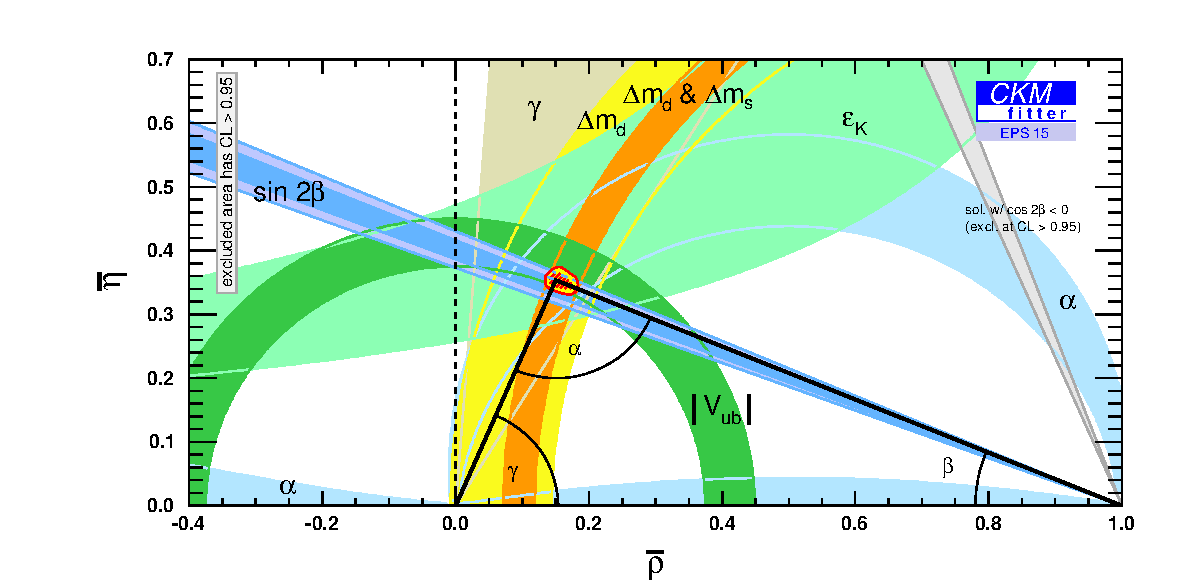
\includegraphics[width=\textwidth]{03-CPViolation/figs/CKMfitterTriangle.pdf}
\caption{Unitarity triangle with constraints from measurements of various
quantities~\cite{CKMfitter}.}
\label{fig:cpviolation:ckmtriangle_fitted}
\end{figure}


%!TEX root = ../main.tex

\section{The system of neutral \texorpdfstring{$\Bd$}{B0} mesons (3 pages)}
\label{sec:cpviolation:neutralBmesons}

%!TEX root = ../main.tex

\section{Types of \texorpdfstring{$\CP$}{CP} violation}
\label{sec:cpviolation:types}

There are three different manifestations of \CP violation. It can occur, when
the decay amplitudes differ between \CP conjugated processes (see
\cref{sec:cpviolation:types:direct}), when the mass eigenstates are no \CP
eigenstates (see \cref{sec:cpviolation:types:indirect}), and when there is
interference between direct decays and decays to the same final state after
mixing (see \cref{sec:cpviolation:types:interference}). While the first type
can appear for charged and neutral hadrons, the latter are only possible for
neutral decays.

All types of \CP violation can be summarized with the condition $\lambda_f
\neq 1$.

%!TEX root = ../main.tex

\subsection{Direct \texorpdfstring{$\CP$}{CP} violation}
\label{sec:cpviolation:types:direct}

Two different type of phases can contribute to decay amplitudes, weak phases
and strong phases. Weak phases can enter through the CKM matrix and take the
opposite sign for \Af and \Abarfbar. Strong phases typically appear in
scattering processes and originate from intermediate on-shell states. They
occur with the same sign in \Af and \Abarfbar. However, only phase differences
are physically meaningful, as the SM is a gauge-invariant theory and thus
absolute phases could be removed by a rotation of the system. So, at least two
terms with different weak and strong phases need to contribute to the decay
amplitudes to have an effect. The superposition of several contributions with
individual magnitudes $A_i$, weak phases $e^{i\phi_i}$ and strong phases
$e^{i\delta_i}$ leads to
\begin{align}
\begin{split}
	\Af = &\sum_i A_i e^{i(\delta_i+\phi_i)}\,,\\
	\Abarfbar = e^{2i(\xi_f-\xi_B)}&\sum_i A_i e^{i(\delta_i-\phi_i)}\,,
\end{split}
\end{align}
where $\xi_f$ and $\xi_B$ are arbitrary phases coming from the \CP
transformation on the \Bd meson and the final state, respectively. If the
final state $f$ is a \CP eigenstate, the term $e^{2i\xi_f} = \num{\pm1}$
represents the \CP eigenvalue. Direct \CP violation is present for
\begin{align}
	\left|\frac{\Abarfbar}{\Af}\right| = \left|\frac{\sum A_i e^{i(\delta_i-\phi_i)}}{\sum A_i e^{i(\delta_i+\phi_i)}}\right| \neq 1\,.
\end{align}

This type of \CP violation is observed in charmless two-body decays of neutral
$B$ mesons~\cite{Lees:2012mma,Duh:2012ie,LHCb-PAPER-2013-018}.

%!TEX root = ../main.tex

\subsection{Indirect \texorpdfstring{$\CP$}{CP} violation}
\label{sec:cpviolation:types:indirect}

Indirect \CP violation occurs when the mass eigenstates are no \CP eigenstates
and instead a relative phase is present between $M_{12}$ and $\Gamma_{12}$.
Following \cref{eq:cpviolation:neutralBmesons:qp} this means
\begin{align}
	\left|\frac qp \right| \neq 1\,.
\end{align}
So, it can be interpreted as difference of the mixing probabilities between
\Bd and \Bdb mesons
\begin{align}
	\mathcal{P}(\Bd\!\to\Bdb,t) \neq \mathcal{P}(\Bdb\!\to\Bd,t)\,,
\end{align}
and thus is also called \CP violation in mixing. While this type of \CP
violation has been observed in the system of neutral kaons, all measurements
in the system of neutral $B$ mesons yield values for the asymmetry of
semileptonic decays
\begin{align}
	a_{\mathrm{sl}} = \frac{\Gamma(\Bdb(t)\!\to\ellp\nu X) - \Gamma(\Bd(t)\!\to\ellm\nu X)}{\Gamma(\Bdb(t)\!\to\ellp\nu X) + \Gamma(\Bd(t)\!\to\ellm\nu X)} = \frac{1 - |q/p|^4}{1 + |q/p|^4}
\end{align}
consistent with zero~\cite{LHCb-PAPER-2014-053,LHCb-PAPER-2016-013}, though
the precision is one to two magnitudes above the SM expectations. This lack in
precision is not only due to statistical uncertainties. When extracting the
\CP asymmetry from the raw asymmetry further asymmetries, like detection and
production asymmetries, need to be taken into account, and these are not
precisely known.

%!TEX root = ../main.tex

\subsection{\texorpdfstring{$\CP$}{CP} violation in the interference of decay and decay after mixing (2 pages)}
\label{sec:cpviolation:types:interference}

%!TEX root = ../main.tex

\section{\texorpdfstring{$\CP$}{CP} violation in \texorpdfstring{$\bToccbars$}{bToccbars} decays (2 pages)}
\label{sec:cpviolation:btoccbars}

The gold-plated mode to measure \CP violation in the system of neutral $B$
mesons is \BdToJPsiKS. It proceeds via a \bToccbars transition. Direct and
indirect \CP violation is strongly suppressed, which makes it a very clean
mode to determine the weak mixing phase, and thus the CKM angle $\beta$, via
\CP violation in the interference of decay and decay after mixing. As the
Feynman diagrams in \cref{fig:cpviolation:bd2jpsiks_feynmans} show, actually
\BdToJPsiKz and \BdbToJPsiKzb decays take place.
\begin{figure}[htb]
\centering
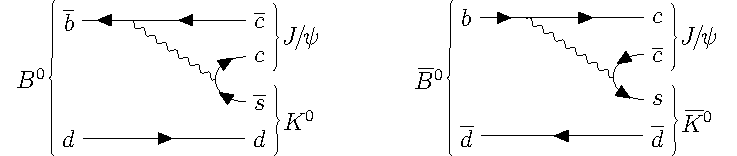
\includegraphics[width=\textwidth]{03-CPViolation/tikz/pdf/BdToJPsiKS_Feynmans.pdf}
\caption{Tree Feynman diagrams of \BdToJPsiKS for both flavours.}
\label{fig:cpviolation:bd2jpsiks_feynmans}
\end{figure}
However, like for the $B$ mesons the flavour eigenstates are a superposition
of the \CP mass eigenstates:
\begin{align}
	\ket{\KS} = p_K \ket{\Kz} - q_K \ket{\Kzb}
\end{align}
Therefore, the ratio of decay amplitudes is composed of two terms according to
\begin{align}
	\frac{\bar{A}_{\JPsi\KS}}{A_{\JPsi\KS}} = -\frac{p_K}{q_K}\frac{\bar{A}_{\JPsi\Kzb}}{A_{\JPsi\Kz}}\,.
\end{align}
The ratio of the mixing coefficients for the kaons can be calculated using
\cref{eq:cpviolation:qp}. Different than for the $B$ mesons the dominant
contribution to the mixing diagrams arises from charm quarks in the loop:
\begin{align}
	\frac{p_K}{q_K} = -\frac{\Vcs\Vcds}{\Vcss\Vcd}
\end{align}
Accounting only for the tree diagrams in
\cref{fig:cpviolation:bd2jpsiks_feynmans}, while neglecting loop processes,
the ratio of the direct decay amplitudes can be expressed via the involved CKM
matrix elements:
\begin{align}
	\frac{\bar{A}_{\JPsi\Kzb}}{A_{\JPsi\Kz}} = \frac{\Vcb\Vcss}{\Vcbs\Vcs}
\end{align}
Summarising these values and adding the ratio of CKM matrix elements for the
mixing of the \Bd mesons (see \cref{eq:cpviolation:qp_simplified}) the
parameter describing \CP violation from \cref{eq:cpviolation:lambda} becomes
\begin{align}
	\lambda_{\JPsi\KS} = - \frac{\Vtbs\Vtd}{\Vtb\Vtds}\frac{\Vcs\Vcds}{\Vcss\Vcd}\frac{\Vcb\Vcss}{\Vcbs\Vcs} = - \frac{\Vtbs\Vtd}{\Vtb\Vtds}\frac{\Vcds\Vcb}{\Vcd\Vcbs}
\end{align}
The minus sign indicates that the final state $\JPsi\KS$ is \CP-odd, as an
angular momentum of $l = 1$ is necessary to compensate that the \Bd meson as
initial state has spin zero, while the final state consists of a \CP-even
$\JPsi$ meson with spin one and an almost \CP-even\footnote{When reconstructed
in a pair of two pions it is fully \CP-even.} \KS meson with spin zero.

%!TEX root = ../main.tex

\section{\texorpdfstring{$\CP$}{CP} violation in \texorpdfstring{$\bToccbard$}{bToccbard} decays}
\label{sec:cpviolation:btoccbard}

The decay \BdToDD can be described with the Feynman diagrams in
\cref{fig:cpviolation:feynmandiagrams_bdtodd}.
\begin{figure}[htb]
\centering
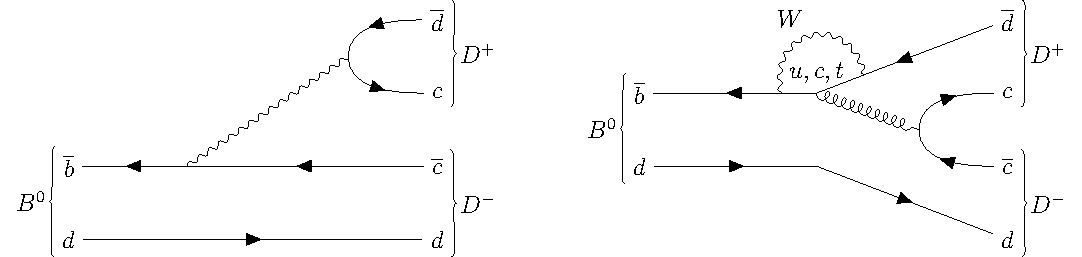
\includegraphics[width=\textwidth]{03-CPViolation/tikz/pdf/BdToDD_Feynmans.pdf}
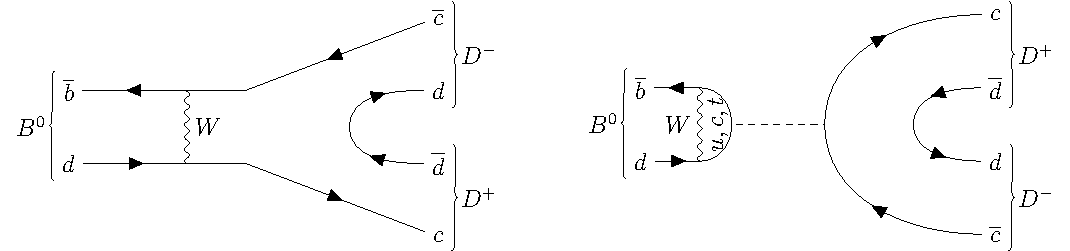
\includegraphics[width=\textwidth]{03-CPViolation/tikz/pdf/BdToDD_Feynmans2.pdf}
\caption{Main Feynman diagrams contributing to \BdToDD decays. Apart from the
tree diagram (top left), a penguin diagram (top right), an exchange diagram
(bottom left) and a penguin annihilation diagram (bottom right) are shown.}
\label{fig:cpviolation:feynmandiagrams_bdtodd}
\end{figure}
\todo{improve quality of Feynman diagrams}
The tree diagram ($T$) proceeds via a \bToccbard quark transition, which is
CKM suppressed. The contributions from the other diagrams, especially the
penguin diagrams ($P^{(q)}$ with $q = \cquark$ and \tquark quarks in the
loop), but also exchange ($E$) and penguin annihilation diagrams
($P\!A^{(q)}$), need to be taken into account as well because they can carry
different weak phases and are not Cabibbo-suppressed. Thus, the decay
amplitude is given by~\cite{Fleischer1999,Fleischer2007,Bel:2015wha}
\begin{align}
	A(\BdToDD) = \Vcb \mathcal{A}[1 - ae^{i\theta}e^{i\gamma}]\,,
\end{align}
with
\begin{align}
	\mathcal{A} \equiv \Vcds[T + E + {P^{(c)} + P\!A^{(c)}} - {P^{(t)} + P\!A^{(t)}}]\,,
\end{align}
and
\begin{align}
	ae^{i\theta} \equiv R_b\left[\frac{{P^{(u)} + P\!A^{(u)}} - {P^{(t)} + P\!A^{(t)}}}{T + E + {{P^{(c)} + P\!A^{(c)}} - {P^{(t)} + P\!A^{(t)}}}}\right]\,.
\end{align}
Here, $R_b$ is a side length of the unitarity triangle defined in
\cref{eq:cpviolation:Rb}. The angle $\gamma$ of the unitarity triangle is a
\CP-violating weak phase, while $a$ and $\theta$ are hadronic \CP-conserving
parameters. Therefore, the corresponding \Bzb decay amplitude is
\begin{align}
	A(\BdbToDD) = \Vcbs \mathcal{A}[1 - ae^{i\theta}e^{-i\gamma}]\,.
\end{align}
The parameter describing \CP violation in the interference can be written as
\begin{align}
\begin{split}
	\lambda_{\Dp\Dm} &= \frac{\Vtbs\Vtd}{\Vtb\Vtds}\frac{\Vcb\Vcds}{\Vcbs\Vcd}\frac{1-ae^{i\theta}e^{i\gamma}}{1-ae^{i\theta}e^{-i\gamma}}\,,\\
					 &= e^{-i2\beta}\frac{1-ae^{i\theta}e^{i\gamma}}{1-ae^{i\theta}e^{-i\gamma}}\,,
\end{split}
\end{align}
using the ratio of the mixing coefficients from
\cref{eq:cpviolation:qp_simplified} and the definition of the unitarity
triangle $\beta$ from \cref{eq:cpviolation:angles}. Different than for
\BdToJPsiKS (cf.~\cref{eq:lambda_JPsiKS}) the \CP eigenvalue is $\eta_{\CP} =
\num{+1}$, since no spins are involved in the decay \BdToDD. The hadronic
parameters cannot be calculated reliably within QCD~\cite{Bel:2015wha}. Thus,
they must be determined through a measurement of the \CP observables, which
can be expressed via
\begin{align}
	\SDD &= -\frac{\sin\phid - 2a \cos\theta\sin(\phid + \gamma) + a^2\sin(\phid + 2\gamma)}{1 - 2a\cos\theta\cos\gamma + a^2}\,,\\
	\CDD &= \frac{2a\sin\theta\sin\gamma}{1 - 2a\cos\theta\cos\gamma + a^2}\,.
\end{align}
The term \SDD gives access to the mixing phase \phid, which is related to $\beta$ through
\begin{align}
	\phid = 2\beta + \phi_d^{\mathrm{NP}}\,,
\end{align}
and thus considers new physics contributions as well. While \SDD is caused by
interference between the direct decay and the decay after mixing, \CDD
might differ from zero due to interferences between tree and penguin
contributions. Different than in the case of \BdToJPsiKS only an effective
phase
\begin{align}
	\phideff = \phid + \Delta\phid
\end{align}
with
\begin{align}
	\sin\phideff = -\frac{\SDD}{\sqrt{1 - \CDD^2}}
\end{align}
can be measured in \BdToDD. The phase shift $\Delta\phi$ is given by
\begin{align}
	\tan\Delta\phi = \frac{a^2\sin2\gamma - 2a\cos\theta\sin\gamma}{1 - 2a\cos\rho\cos\gamma + a^2\cos2\gamma}\,.
\end{align}

The decay channel \BsToDsDs is also governed by a \bToccbard transition. It
gives access to \phis. However, the measurement is as well polluted by
hadronic penguin effects. Since \BsToDsDs is related to \BdToDD via U-spin
symmetry, the phase shift $\Delta\phi$ can be transferred.

Further decay modes from the family of \BToDDbar decays are \BdToDstD and
\BdToDstDst, which also enable a determination of \phideff, but introduce
further complications. For \BdToDstD the final state is no \CP eigenstate as
it can be distinguished by the charge of the \Dstarpm meson. Thus, four \CP
observables are needed to describe \CP violation. Furthermore, from an
experimentalist's point of view the final state is not symmetrical in terms of
the charges of pions and kaons and thus a detection asymmetry has to be taken
into account. In the measurement of \CP violation using \BdToDstDst decays,
like for \BsToJPsiPhi decays, an angular-dependent analysis is required.
